% !TEX root = ../paper.tex

\section{Introduction}
Software code review is an established cost-effective software quality management practice.
Its main intent is to  identify  defects early and encourage quality development practices such as adherence to coding standards and improving code readability.
Nowadays less formal and lightweight code reviews such as Modern Code Review (MCR)\cite{Bacchelli2013a} have received much attention and are commonly used within both industry and OSS projects.
One reason for this is that with MCR, unlike formal inspections \cite{Fagan:1976:DCI:1661010.1661012}, in-person meetings are not required.
Reviewers can find problems in proposed changes and hold discussions on them by adding comments through a code review tool or a mailing list.
Developers then improve the changes in response to these comments and re-submit for review until the changes are approved.  
%Fig. \ref{fig:process} illustrates a typical MCR process. 

Because performance of code review has a clear relationship to the quality of the software, many studies have investigated factors that influence MCR\cite{Baysal2001,Mcintosh,Beller,Hamasaki2013}.
However, little research exists investigating how review discussion for a proposed change impacts software quality.
Given that most proposed changes are triggered from reviewer comments \cite{Beller}, 
it is possible that they can either positively contribute to the proposed changes (i.e. are ``\emph{useful}''), or be a discussion which contributes little directly to the proposed changes (i.e. relatively ``\emph{useless}''). 
Since MCR does not require strict guidelines, checklists, or formal processes, some reviewers tend to look for trivial issues (e.g. coding styles), leaving deeper issues undiscussed \cite{Bacchelli2013a}.
%This is a concern because a high-degree of useless comments not only fails to contribute to improving quality, but also degrades the cost-effectiveness and perceived utility of MCR.
This is a concern because a low-degree of useful comments can degrade the overall quality and perceived utility of MCR.

Prior research has focused mostly on the relation between number of comments and quality.
To the best of our knowledge, the connection between degree of useful and useless comments and quality has not been studied.
One reason for this may be that to assess the impact of discussion in MCR, effort-intensive manual classification is required as in the study of Beller et. al. \cite{Beller}.
MCR can produce a massive amounts of changes requests and comments\cite{Balachandran2013,Thongtanunam2014} and it is painstaking and time consuming to classify their usefulness.
Moreover, comments in MCR are unstructured natural text, open to subjective judgment, tacit understanding, and possible misinterpretation. 



% Fig. \ref{fig:example} show typical MCR comments illustrating these issues.
%Moreover, unlike a checklist in used formal inspection, the comments in MCR are unstructured natural text, open to subjective judgment, tacit understanding, and possible mis-interpretation.  Fig. \ref{fig:example} show typical MCR comments illustrating these issues.




In this paper, we present a text mining approach using semantic similarity to assist in classifying the usefulness of comments.
The proposed approach is meant to ease classifying large amounts of MRC comments in order to conduct comment and code quality studies (such as those discussed earlier) as manual classification can quickly become an untenable task.
By introducing automation support based on objective empirical criteria, our proposed method aims to both reduce effort and increase confidence in classification to a degree that is practical for addressing very large MRC data sets.
%Because usefulness of a comment is not precisely defined and is a subjective qualification, we cannot, and do not intend to fully automate or replace human driven classification.  
Through a case study of Qt project, we address the following research questions:
\begin{ResearchQuestions}
\item[RQ1:] Is semantic similarity a good indicator of MCR comment usefulness?\\
\item[RQ2:] Is semantic similarity classification cost-efficient, assurable, and scalable?
\end{ResearchQuestions}

Our contributions are as follows:
\begin{itemize}
\item We propose a practical approach to mine natural text of comments in code reviews and classify their usefulness using semantic similarity.
\item We investigate relationship between usefulness of comments and semantic similarity.
\item We investigate cost-efficient, assurable and scalable of semantic similarity in large open source project based on actual human effort.
\end{itemize}

%%%%%%%%% TEMP %%%%%%%%%
%\dan{Much of the following material should be placed in a separate Motivation section} 

%We define a \emph{useful} comment as one that \emph{contributes to improving the proposed changes} and a \emph{useless}\footnote{Although we call these comments \emph{useless}, it might be useful---or sometimes even required---in some other context, such as to facilitate communication.} comment as one that does not.
%Usefulness is not dichotomous and hence we must accept a third qualification, \emph{unclear}, to allow for the case where a comment does not directly make a positive contribution but is not clearly out of scope or tangential.

%In our approach, we analyze the similarity between a commit message of the proposed changes and the respective comments that follow.

%Our key idea is that useful comments are likely to have a strong semantic similarity to the proposed changes, while useless comments are more likely strongly dissimilar.
%To determine these semantic relationships, we use the Vector Space Model (VSM) and calculate similarity (using cosine similarity) and dissimilarity (using euclidean distance) between the comment and commit message vectors. 

%We create our predictive model by estimating pairs of similarity and dissimilarity values that best discriminate between useful and useless comments.
%This is accomplished by optimizing for prediction performance measures such as Precision and Recall, through F-measure.
%
%For our case study of the method, we used a review history from the Gerrit\footnote{\url{https://code.google.com/p/gerrit/}} system from Qt\footnote{\url{http://qt-project.org/}}, an open source project for a cross-platform application and UI framework supported by Digia corporation.
%For training and validation of our approach, three experts manually classified the usefulness for 320 comments.
%We also apply our predictive model to the full set of 17,000 \dan{what's the actual number?}
%comments to obtain a preliminary estimate in the quality of reviews and address the following three research questions:
%
%\noindent \textbf{RQ1:} Is semantic similarity a good indicator of MCR comment usefulness?\\
%\noindent \textbf{RQ2:} Do code reviewers intensively discuss on the proposed changes?\\
%\noindent \textbf{RQ3:} Is semantic similarity classification cost-efficient, assurable, and scalable?
%
%\noindent In addition to addressing the research questions above, the main contributions of this paper are:
%\dan{these are more "results" than contributions.... need to reword this!}
%\begin{itemize}
%\item A practical approach to mine natural text of comments in code reviews and classify their usefulness based on VSM similarity.
%\item The experimental results, which show that the approach can classify comments with an F$_1$ score of 0.681 and 0.693.
%\item 
%\item \TODO{xx}\% of the comments did not have unanimity (i.e. unclear), and of these \TODO{yy}\% were automatically determined to be useful or not useful. Follow up with dissenting assessors found mis-judgement occurred \TODO{zz}\% of the time whereby in retrospect the comment would have had unanimity. This indicates the method is useful in identifying subjective judgement errors. 
%\item Of the 23\% not automatically classified (i.e. undetermined), \TODO{qq}\% were unclear. Of the \TODO{(1-qq)}\% with unanimity, followup with assessors found in retrospect they would change their assessment making the comment unclear. This indicates the method is useful in identifying chance unanimity errors or group think bias.
%\end{itemize} 
%%%%%%%%%%%%%%%%%%%%%%%%%%%

%Software Inspection is basically composed of a three-step procedure: preparation, inspection meeting, and repair.

\begin{figure}[!t]
\centering
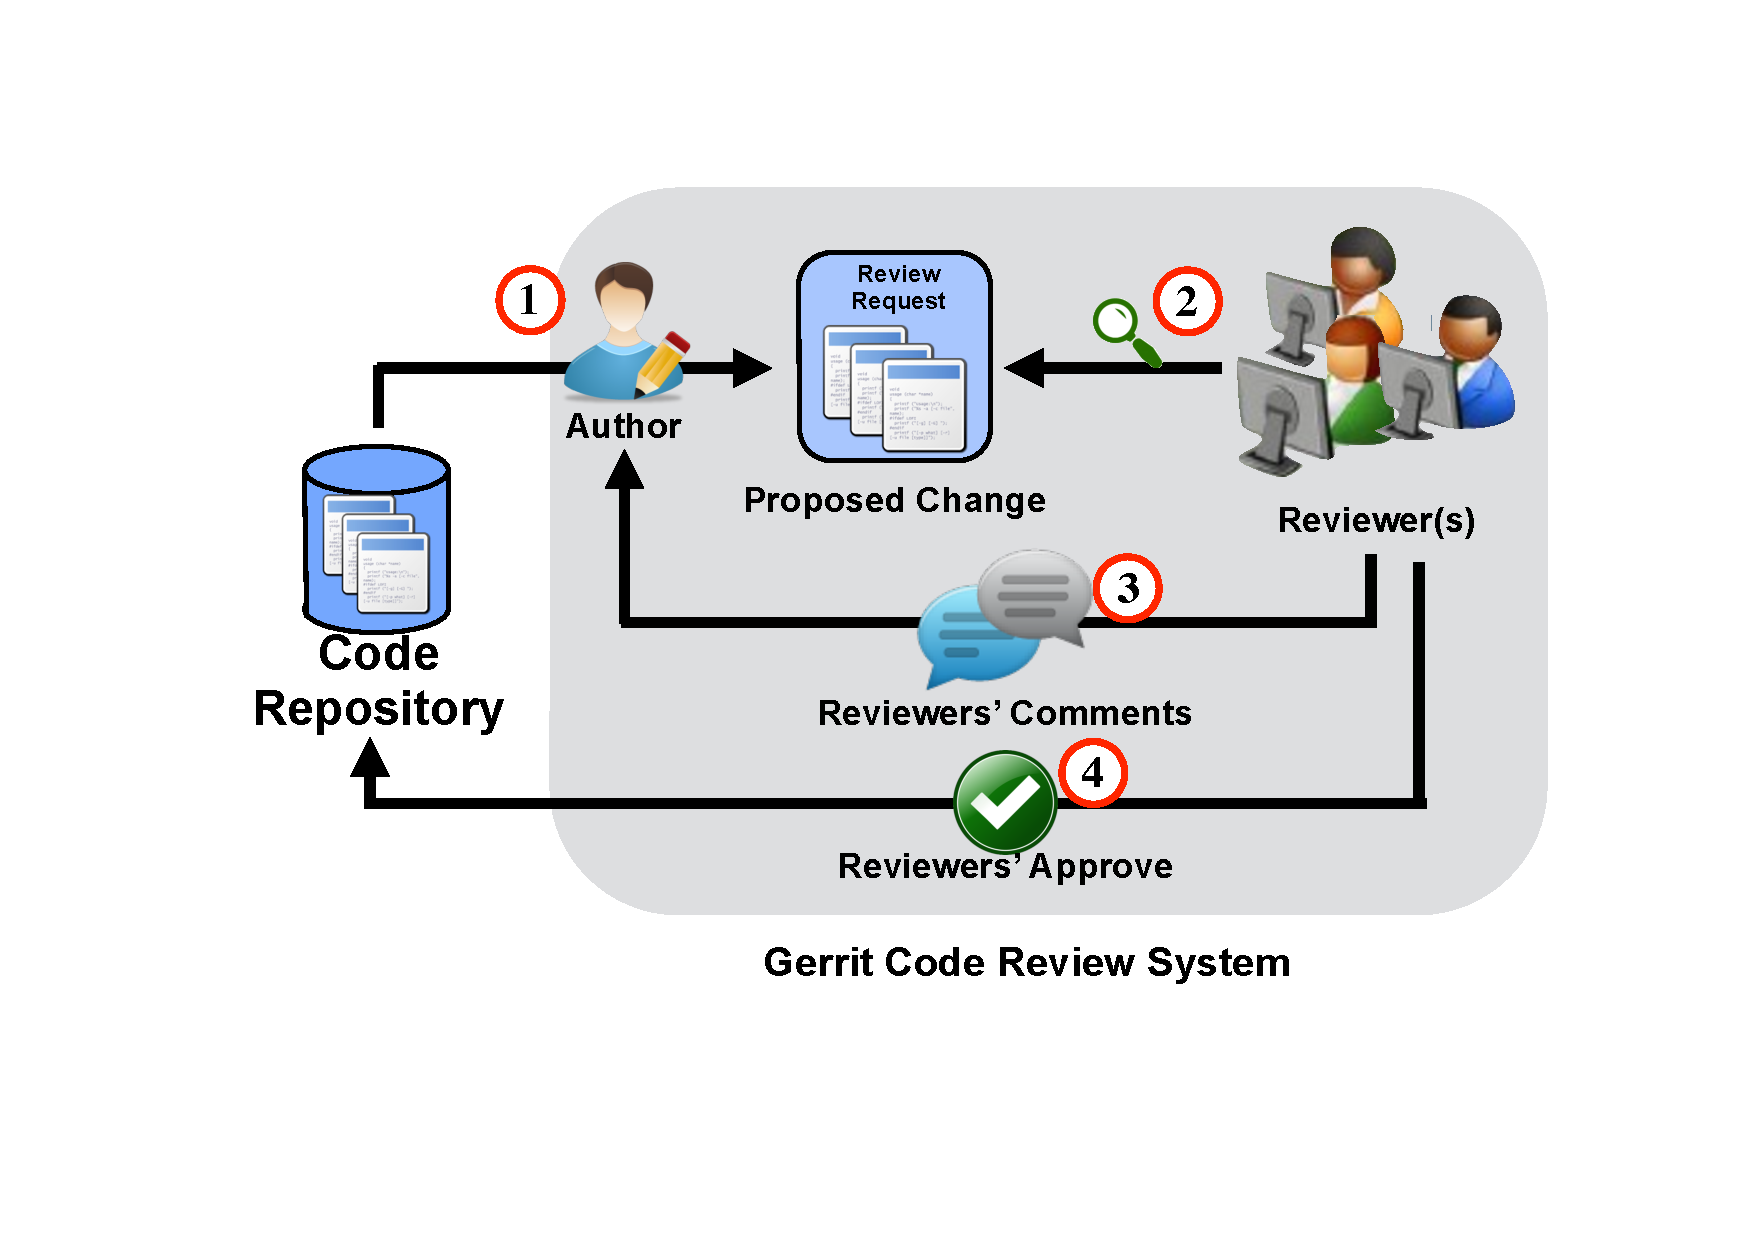
\includegraphics[scale=0.35, trim= 100 110 50 80, clip=true]{review_process}
\caption{An simplified version of MCR Process based on Gerrit system}
\label{fig:process}
\end{figure}